\documentclass[openany]{book}
\usepackage{amsmath, amssymb, graphicx,hyperref}
\begin{document}
%\title{}
%\author{Alec Mouri}
%\maketitle
\frontmatter
\tableofcontents
\mainmatter
\chapter{Matrices}
%Section 1: 
\section{The Basic Operations}
%\section*{Exercises}
\begin{description}
\item[(1.1/1.1)]
$a_{21} = 2, s_{23} = 8$
\item[(1.2)]
\begin{itemize}
\item[(a)]
$$AB = \begin{bmatrix}
1 & 2 & 3 \\
3 & 3 & 1
\end{bmatrix}\begin{bmatrix}
-8 & -4 \\
9 & 5 \\
-3 & -2
\end{bmatrix} = \begin{bmatrix}
1 & 0 \\
0 & 1
\end{bmatrix}$$
$$BA = \begin{bmatrix}
-8 & -4 \\
9 & 5 \\
-3 & -2
\end{bmatrix}\begin{bmatrix}
1 & 2 & 3 \\
3 & 3 & 1
\end{bmatrix} = \begin{bmatrix}
-20 & -28 & - 28 \\
24 & 33 & 33 \\
-9 & -12 & -11
\end{bmatrix}$$
\item[(b)]
$$AB = \begin{bmatrix}
1 & 4 \\
1 & 2
\end{bmatrix}\begin{bmatrix}
6 & -4 \\
-3 & 2
\end{bmatrix} = \begin{bmatrix}
-6 & -4 \\
0 & 0
\end{bmatrix}$$
$$BA = \begin{bmatrix}
6 & -4 \\
-3 & 2
\end{bmatrix}\begin{bmatrix}
1 & 4 \\
1 & 2
\end{bmatrix} = \begin{bmatrix}
2 & 16 \\
-1 & -8
\end{bmatrix}$$
\item[(c)]
$$AB = \begin{bmatrix}
1 \\
-1 \\
0
\end{bmatrix}\begin{bmatrix}
1 & 2 & 1
\end{bmatrix} = \begin{bmatrix}
1 & 2 & 1 \\
-1 & -2 & -1 \\
0 & 0 & 0
\end{bmatrix}$$
$$BA = \begin{bmatrix}
1 & 2 & 1
\end{bmatrix}\begin{bmatrix}
1 \\
-1 \\
0
\end{bmatrix} = \begin{bmatrix}
-1
\end{bmatrix}$$
\end{itemize}
\item[(1.3)]
$$AB = \begin{bmatrix}
a_1 & \hdots & a_n
\end{bmatrix}\begin{bmatrix}
b_1 \\
\vdots \\
b_n
\end{bmatrix} = \begin{bmatrix}
a_1b_1 + ... + a_nb_n
\end{bmatrix}$$
$$BA = \begin{bmatrix}
b_1 \\
\vdots \\
b_n
\end{bmatrix}\begin{bmatrix}
a_1 & \hdots & a_n
\end{bmatrix} = \begin{bmatrix}
a_1b_1 & a_2b_1 & \hdots & a_nb_1 \\
a_1b_2 & a_2b_2 & \hdots & a_nb_2 \\
\vdots & \vdots & \ddots & \vdots \\
a_1b_n & a_2b_n & \hdots & a_nb_n
\end{bmatrix}$$
\item[(1.4)]
$$\left( \begin{bmatrix}
1 & 2 \\
0 & 1
\end{bmatrix}\begin{bmatrix}
0 & 1 & 2 \\
1 & 1 & 3
\end{bmatrix} \right)\begin{bmatrix}
1 \\
4 \\
3
\end{bmatrix} = \begin{bmatrix}
2 & 3 & 8 \\
1 & 1 & 3
\end{bmatrix}\begin{bmatrix}
1 \\
4 \\
3
\end{bmatrix} = \begin{bmatrix}
38 \\
14
\end{bmatrix}$$
$$\begin{bmatrix}
1 & 2 \\
0 & 1
\end{bmatrix} \left(\begin{bmatrix}
0 & 1 & 2 \\
1 & 1 & 3
\end{bmatrix}\begin{bmatrix}
1 \\
4 \\
3
\end{bmatrix} \right) = \begin{bmatrix}
1 & 2 \\
0 & 1
\end{bmatrix}\begin{bmatrix}
10 \\
14
\end{bmatrix} = \begin{bmatrix}
38 \\
14
\end{bmatrix}$$
\item[(1.5)]
$$\begin{bmatrix}
1 & a \\
& 1
\end{bmatrix}\begin{bmatrix}
1 & b \\
& 1
\end{bmatrix} = \begin{bmatrix}
1 & a + b \\
& 1
\end{bmatrix}$$
\item[(1.6)]
I claim that
$$\begin{bmatrix}
1 & 1 \\
& 1
\end{bmatrix}^n = \begin{bmatrix}
1 & n \\
& 1
\end{bmatrix}$$
Let $n = 1$. Then
$$\begin{bmatrix}
1 & 1 \\
& 1
\end{bmatrix}$$
So the statement is trivially true for $n = 1$. Suppose the statement is true for $n = k - 1$. Then
$$\begin{bmatrix}
1 & 1 \\
& 1
\end{bmatrix}^k = \begin{bmatrix}
1 & 1 \\
& 1
\end{bmatrix}^{k-1}\begin{bmatrix}
1 & 1 \\
& 1
\end{bmatrix} = \begin{bmatrix}
1 & k - 1 \\
& 1
\end{bmatrix}\begin{bmatrix}
1 & 1 \\
& 1
\end{bmatrix} = \begin{bmatrix}
1 & k \\
& 1
\end{bmatrix}$$
\item[(1.7)]
I claim that
$$\begin{bmatrix}
1 & 1 & 1 \\
& 1 & 1 \\
& & 1
\end{bmatrix}^n = \begin{bmatrix}
1 & n & T_n \\
& 1 & n \\
& & 1
\end{bmatrix}$$
Where $T_n = \sum_{i=1}^n i$

Suppose $n = 1$. Then
$$\begin{bmatrix}
1 & 1 & 1 \\
& 1 & 1 \\
& & 1
\end{bmatrix}^n = \begin{bmatrix}
1 & 1 & 1 \\
& 1 & 1 \\
& & 1
\end{bmatrix}$$
Since $T_1 = 1$, then the statement is true. Suppose the statement is true for $n = k - 1$. Then
\begin{align*}
\begin{bmatrix}
1 & 1 & 1 \\
& 1 & 1 \\
& & 1
\end{bmatrix}^k & = \begin{bmatrix}
1 & 1 & 1 \\
& 1 & 1 \\
& & 1
\end{bmatrix}^{k-1}\begin{bmatrix}
1 & 1 & 1 \\
& 1 & 1 \\
& & 1
\end{bmatrix}		\\
&= \begin{bmatrix}
1 & k-1 & T_{k-1} \\
& 1 & k-1 \\
& & 1
\end{bmatrix}\begin{bmatrix}
1 & 1 & 1 \\
& 1 & 1 \\
& & 1
\end{bmatrix} = \begin{bmatrix}
1 & k-1 + 1 & T_{k-1} + k-1 + 1 \\
& 1 & k -1 + 1 \\
& & 1 
\end{bmatrix}\\
& = \begin{bmatrix}
1 & k & T_k \\
& 1 & k \\
& & 1
\end{bmatrix}
\end{align*}
$$\begin{bmatrix}
1 & 1 & 1 \\
& 1 & 1 \\
& & 1
\end{bmatrix}^k = \begin{bmatrix}
1 & 1 & 1 \\
& 1 & 1 \\
& & 1
\end{bmatrix}^{k-1}\begin{bmatrix}
1 & 1 & 1 \\
& 1 & 1 \\
& & 1
\end{bmatrix}$$
$$ = \begin{bmatrix}
1 & k-1 & T_{k-1} \\
& 1 & k-1 \\
& & 1
\end{bmatrix}\begin{bmatrix}
1 & 1 & 1 \\
& 1 & 1 \\
& & 1
\end{bmatrix} = \begin{bmatrix}
1 & k-1 + 1 & T_{k-1} + k-1 + 1 \\
& 1 & k -1 + 1 \\
& & 1 
\end{bmatrix}$$
$$= \begin{bmatrix}
1 & k & T_k \\
& 1 & k \\
& & 1
\end{bmatrix}$$
\item[(1.8)]
$$\begin{bmatrix} 
\begin{array}{cc|cc}
1 & 1 & 1 & 5 \\
0 & 1 & 0 & 1 \\
\hline
1 & 0 & 0 & 1 \\
0 & 1 & 1 & 0
\end{array}
\end{bmatrix}\begin{bmatrix} 
\begin{array}{cc|cc}
1 & 2 & 1 & 0 \\
0 & 1 & 0 & 1 \\
\hline
1 & 0 & 0 & 1 \\
0 & 1 & 1 & 3
\end{array}
\end{bmatrix}$$
$$= \begin{bmatrix}
\begin{array}{c|c}

\begin{bmatrix}
1 & 1 \\
0 & 1
\end{bmatrix} \begin{bmatrix}
1 & 2 \\
0 & 1
\end{bmatrix} + \begin{bmatrix}
1 & 5 \\
0 & 1
\end{bmatrix}\begin{bmatrix}
1 & 0 \\
0 & 1
\end{bmatrix} & \begin{bmatrix}
1 & 1 \\
0 & 1
\end{bmatrix} \begin{bmatrix}
1 & 0 \\
0 & 1
\end{bmatrix} + \begin{bmatrix}
1 & 5 \\
0 & 1
\end{bmatrix}\begin{bmatrix}
0 & 1 \\
1 & 3
\end{bmatrix} \\
\hline
\begin{bmatrix}
1 & 0 \\
0 & 1
\end{bmatrix} \begin{bmatrix}
1 & 2 \\
0 & 1
\end{bmatrix} + \begin{bmatrix}
0 & 1 \\
1 & 0
\end{bmatrix}\begin{bmatrix}
1 & 0 \\
0 & 1
\end{bmatrix} & \begin{bmatrix}
1 & 0 \\
0 & 1
\end{bmatrix} \begin{bmatrix}
1 & 0 \\
0 & 1
\end{bmatrix} + \begin{bmatrix}
0 & 1 \\
1 & 0
\end{bmatrix}\begin{bmatrix}
0 & 1 \\
1 & 3
\end{bmatrix}
\end{array}
\end{bmatrix}$$
$$= \begin{bmatrix}
\begin{array}{c|c}
\begin{bmatrix}
1 & 3 \\
0 & 1
\end{bmatrix} + \begin{bmatrix}
1 & 5 \\
0 & 1
\end{bmatrix} & \begin{bmatrix}
1 & 1 \\
0 & 1
\end{bmatrix} + \begin{bmatrix}
5 & 16 \\
1 & 3
\end{bmatrix} \\
\hline
\begin{bmatrix}
1 & 2 \\
0 & 1
\end{bmatrix} + \begin{bmatrix}
0 & 1 \\
1 & 0
\end{bmatrix} & \begin{bmatrix}
1 & 0 \\
0 & 1
\end{bmatrix} + \begin{bmatrix}
1 & 3 \\
0 & 1
\end{bmatrix}
\end{array}
\end{bmatrix} = \begin{bmatrix}
2 & 8 & 6 & 17 \\
0 & 2 & 1 & 4 \\
1 & 3 & 2 & 3 \\
1 & 1 & 0 & 1
\end{bmatrix}$$
$$\begin{bmatrix} 
\begin{array}{c|cc}
0 & 1 & 2 \\
\hline
0 & 1 & 0 \\
3 & 0 & 1
\end{array}
\end{bmatrix}\begin{bmatrix} 
\begin{array}{c|cc}
1 & 2 & 3 \\
\hline
4 & 2 & 3 \\
5 & 0 & 4
\end{array}
\end{bmatrix}$$
$$= \begin{bmatrix} 
\begin{array}{c|c}
\begin{bmatrix}
0
\end{bmatrix}\begin{bmatrix}
1
\end{bmatrix} + \begin{bmatrix}
1 & 2
\end{bmatrix}\begin{bmatrix}
4 \\
5
\end{bmatrix} & \begin{bmatrix}
0
\end{bmatrix}\begin{bmatrix}
2 & 3
\end{bmatrix} + \begin{bmatrix}
1 & 2
\end{bmatrix}\begin{bmatrix}
2 & 3 \\
0 & 4
\end{bmatrix} \\
\hline
\begin{bmatrix}
0 \\
3
\end{bmatrix}\begin{bmatrix}
1
\end{bmatrix} + \begin{bmatrix}
1 & 0 \\
0 & 1
\end{bmatrix}\begin{bmatrix}
4 \\
5
\end{bmatrix} & \begin{bmatrix}
0 \\
3
\end{bmatrix}\begin{bmatrix}
2 & 3
\end{bmatrix} + \begin{bmatrix}
1 & 0 \\
0 & 1
\end{bmatrix}\begin{bmatrix}
2 & 3 \\
0 & 4
\end{bmatrix}
\end{array}
\end{bmatrix}$$
$$= \begin{bmatrix}
\begin{array}{c|c}
\begin{bmatrix}
0
\end{bmatrix} + \begin{bmatrix}
14
\end{bmatrix} & \begin{bmatrix}
0 & 0
\end{bmatrix} + \begin{bmatrix}
2 & 11
\end{bmatrix} \\
\hline
\begin{bmatrix}
0 \\
3
\end{bmatrix} + \begin{bmatrix}
4 \\
5
\end{bmatrix} & \begin{bmatrix}
0 & 0 \\
6 & 9
\end{bmatrix} + \begin{bmatrix}
2 & 3 \\
0 & 4
\end{bmatrix}
\end{array}
\end{bmatrix} = \begin{bmatrix}
14 & 2 & 11 \\
4 & 2 & 3 \\
8 & 6 & 13
\end{bmatrix}$$
%\item[(1.9)]
%Let $M$ be a $m \times n$ matrix and $M'$ be a $n \times p$ matrix where 
%$$M = \begin{bmatrix}
%\begin{array}{c|c}
%A & B \\
%\hline
%C & D
%\end{array}
%\end{bmatrix} = \begin{bmatrix}
%\begin{array}{cccc|cccc}
%a_{11} & a_{12} & \hdots & a_{1i} & b_{11} & b_{12} & \hdots & b_{1 n-i} \\
%a_{21} & a_{22} & \hdots & a_{2i} & b_{21} & b_{22} & \hdots & b_{2 n-i} \\
%\vdots & \vdots & \ddots & \vdots & \vdots & \vdots & \ddots & \vdots \\
%a_{j1} & a_{j2} & \hdots & a_{ji} & b_{j1} & b_{j2} & \hdots & b_{j n-i} \\
%\hline
%c_{11} & c_{12} & \hdots & c_{1i} & d_{11} & d_{12} & \hdots & d_{1 n-i} \\
%c_{21} & c_{22} & \hdots & c_{2i} & d_{21} & d_{22} & \hdots & d_{2 n-i} \\
%\vdots & \vdots & \ddots & \vdots & \vdots & \vdots & \ddots & \vdots \\
%c_{m-j 1} & c_{m-j 2} & \hdots & c_{m-j i} & d_{m-j 1} & d_{m-j 2} & \hdots & d_{m-j n-i} \\
%\end{array}
%\end{bmatrix}$$
%$$M' = \begin{bmatrix}
%\begin{array}{c|c}
%A' & B' \\
%\hline
%C' & D'
%\end{array}
%\end{bmatrix} = \begin{bmatrix}
%\begin{array}{cccc|cccc}
%a'_{11} & a'_{12} & \hdots & a'_{1x} & b'_{11} & b'_{12} & \hdots & b'_{1 p-x} \\
%a'_{21} & a'_{22} & \hdots & a'_{2x} & b'_{21} & b'_{22} & \hdots & b'_{2 p-x} \\
%\vdots & \vdots & \ddots & \vdots & \vdots & \vdots & \ddots & \vdots \\
%a'_{i1} & a'_{i2} & \hdots & a'_{ix} & b'_{i1} & b'_{i2} & \hdots & b'_{i p-x} \\
%\hline
%c'_{11} & c'_{12} & \hdots & c'_{1x} & d'_{11} & d'_{12} & \hdots & d'_{1 p-x} \\
%c'_{21} & c'_{22} & \hdots & c'_{2x} & d'_{21} & d'_{22} & \hdots & d'_{2 p-x} \\
%\vdots & \vdots & \ddots & \vdots & \vdots & \vdots & \ddots & \vdots \\
%c'_{n-i 1} & c'_{n-i 2} & \hdots & c'_{n-i x} & d'_{n-i 1} & d'_{n-i 2} & \hdots & d'_{n-i p-x} \\
%\end{array}
%\end{bmatrix}$$
%Then
%$$MM' = \begin{bmatrix}
%\sum_{k=1}^i a_{1k}a'_{k1} + \sum_{k=1}^{n-i} b_{1k}c'_{k1} & \hdots & \sum_{k=1}^i a_{1k}b'_{k p-x} + \sum_{k=1}^{n-i} b_{1k}d'_{k p-x} \\
%\vdots & \ddots & \vdots \\
% \sum_{k=1}^i c_{1k}a'_{k1} + \sum_{k=1}^{n-i} d_{1k}c'_{k1} & \hdots & \sum_{k=1}^i c_{1k}b'_{k p-x} + \sum_{k=1}^{n-i} d_{1k}d'_{k p-x}
%\end{bmatrix}$$
%$$= \begin{bmatrix}
%\begin{array}{c|c}
%AA' + AC' & A'B + BD' \\
%\hline
%CA' + DC' & CB' + DD'
%\end{array}
%\end{bmatrix}$$
\item[(1.9)]
\begin{itemize}
\item[(a)]
$$A^2 - B^2 = (A + B)(A - B) = A^2 + BA - AB - B^2 \rightarrow BA = AB$$
\item[(b)]
$$(A + B)^3 = (A + B)(A^2 + AB + BA + B^2)$$
$$= A^3 + A^2B + ABA + AB^2 + BA^2 + BAB + B^2A + B^3$$
\end{itemize}
\item[(11)]
\begin{itemize}
\item[(a)]
$$DA = \begin{bmatrix}
d_1a_{11} & d_1a_{12} & \hdots & d_1a_{1n} \\
d_2a_{21}& d_2a_{22} & \hdots & d_2a_{2n} \\
\vdots & \vdots & \ddots & \vdots \\
d_na_{n1} & d_na_{n2} & \vdots & d_na_{nn}
\end{bmatrix}$$
$$AD = \begin{bmatrix}
d_1a_{11} & d_2a_{12} & \hdots & d_na_{1n} \\
d_1a_{21} & d_2a_{22} & \hdots & d_na_{2n} \\
\vdots & \vdots & \ddots & \vdots \\
d_1a_{n1} & d_2a_{n2} & \hdots & d_na_{nn}
\end{bmatrix}$$
\item[(b)]
Let $D, D'$ be $n \times n$ diagonal matrices with entries $d_{ii}$ and $d'_{ii}$ respectively. Then
$$DD' = \begin{bmatrix}
d_{11}d'_{11} & & & \\
& d_{22}d'_{22} & & \\
& & \ddots & \\
& & & d_{nn}d'_{nn}
\end{bmatrix}$$
\item[(c)]
From part (a), each diagonal entry $i$ of either product $DA$ or $AD$ equals $d_ia_{ii}$. If $A$ is an inverse of $D$, then each $d_ia_{ii} = 1$, implying each diagonal entry of $D$ must be nonzero.
\end{itemize}
\item[(12)]
Let $A, B$ be $n \times n$ upper triangular matrices. Then
$$(AB)_{ij} = \sum_{k=1}^n a_{ik}b_{kj} = \sum_{k=i}^j a_{ik}b_{kj}$$
Since $i > j$, then $(AB)_{ij} = 0$. Therefore, $AB$ is upper triangular.
\item[(13)]
\begin{itemize}
\item[(a)]
$$\begin{bmatrix}
1 & 0 \\
0 & 0
\end{bmatrix}\begin{bmatrix}
a & b \\
c & d
\end{bmatrix} = \begin{bmatrix}
a & b \\
c & d
\end{bmatrix}\begin{bmatrix}
1 & 0 \\
0 & 0
\end{bmatrix}$$
$$\rightarrow \begin{bmatrix}
a & b \\
0 & 0
\end{bmatrix} = \begin{bmatrix}
a & 0 \\
c & 0
\end{bmatrix}$$
Thus, a matrix that commutes has the form
$$\begin{bmatrix}
a & 0 \\
0 & 0
\end{bmatrix}$$
\item[(b)]
$$\begin{bmatrix}
0 & 1 \\
0 & 0
\end{bmatrix}\begin{bmatrix}
a & b \\
c & d
\end{bmatrix} = \begin{bmatrix}
a & b \\
c & d
\end{bmatrix}\begin{bmatrix}
0 & 1 \\
0 & 0
\end{bmatrix}$$
$$\rightarrow \begin{bmatrix}
c & d \\
0 & 0
\end{bmatrix} = \begin{bmatrix}
0 & a \\
0 & c
\end{bmatrix}$$
Thus, a matrix that commutes has the form
$$\begin{bmatrix}
0 & a \\
0 & 0
\end{bmatrix}$$
\item[(c)]
$$\begin{bmatrix}
2 & 0 \\
0 & 6
\end{bmatrix}\begin{bmatrix}
a & b \\
c & d
\end{bmatrix} = \begin{bmatrix}
a & b \\
c & d
\end{bmatrix}\begin{bmatrix}
2 & 0 \\
0 & 6
\end{bmatrix}$$
$$\rightarrow \begin{bmatrix}
2a & 2b \\
6c & 6d
\end{bmatrix} = \begin{bmatrix}
2a & 6b \\
2c & 6d
\end{bmatrix}$$
Thus, a matrix that commutes has the form
$$\begin{bmatrix}
a & 0 \\
0 & d
\end{bmatrix}$$
\item[(d)]
$$\begin{bmatrix}
1 & 3 \\
0 & 1
\end{bmatrix}\begin{bmatrix}
a & b \\
c & d
\end{bmatrix} = \begin{bmatrix}
a & b \\
c & d
\end{bmatrix}\begin{bmatrix}
1 & 3 \\
0 & 1
\end{bmatrix}$$
$$\rightarrow \begin{bmatrix}
a + 3c & b + 3d \\
c & d
\end{bmatrix} = \begin{bmatrix}
a & 3a + b \\
c & 3c + d
\end{bmatrix}$$
Thus, a matrix that commutes has the form
$$\begin{bmatrix}
a & b \\
0 & a
\end{bmatrix}$$
\item[(e)]
$$\begin{bmatrix}
2 & 3 \\
0 & 6
\end{bmatrix}\begin{bmatrix}
a & b \\
c & d
\end{bmatrix} = \begin{bmatrix}
a & b \\
c & d
\end{bmatrix}\begin{bmatrix}
2 & 3 \\
0 & 6
\end{bmatrix}$$
$$\rightarrow \begin{bmatrix}
2a + 3c & 2b + 3d \\
6c & 6d
\end{bmatrix} = \begin{bmatrix}
2a & 3a + 6b \\
2c & 3c + 6d
\end{bmatrix}$$
Thus, a matrix that commutes has the form
$$\begin{bmatrix}
a & \frac{3}{4}(d - a) \\
0 & d
\end{bmatrix}$$
\end{itemize}
\item[(14)]
Let $A = (a_{ij})$ be an $n \times n$ matrix. Then
$$0 + A = \begin{bmatrix}
0 & \hdots & 0 \\
\vdots & \ddots & \vdots \\
0 & \hdots & 0
\end{bmatrix} + \begin{bmatrix}
a_{11} & \hdots & a_{1n} \\
\vdots & \ddots & \vdots \\
a_{n1} & \hdots & a_{nn}
\end{bmatrix}$$
$$= \begin{bmatrix}
0 + a_{11} & \hdots & 0 + a_{1n} \\
\vdots & \ddots & \vdots \\
0 + a_{n1} & \hdots & 0 + a_{nn}
\end{bmatrix} = \begin{bmatrix}
a_{11} & \hdots & a_{1n} \\
\vdots & \ddots & \vdots \\
a_{n1} & \hdots & a_{nn}
\end{bmatrix} = A$$
$$0A = \begin{bmatrix}
0 & \hdots & 0 \\
\vdots & \ddots & \vdots \\
0 & \hdots & 0
\end{bmatrix}\begin{bmatrix}
a_{11} & \hdots & a_{1n} \\
\vdots & \ddots & \vdots \\
a_{n1} & \hdots & a_{nn}
\end{bmatrix}$$
$$ = \begin{bmatrix}
0a_{11} + \hdots + 0a_{n1} & \hdots & 0a_{1n} + \hdots + 0a_{nn} \\
\vdots & \ddots & \vdots \\
0a_{11} + \hdots + 0a_{n1} & \hdots & 0a_{1n} + \hdots + 0a_{nn}
\end{bmatrix} = \begin{bmatrix}
0 & \hdots & 0 \\
\vdots & \ddots & \vdots \\
0 & \hdots & 0
\end{bmatrix} = 0$$
$$A0 = \begin{bmatrix}
a_{11} & \hdots & a_{1n} \\
\vdots & \ddots & \vdots \\
a_{n1} & \hdots & a_{nn}
\end{bmatrix}\begin{bmatrix}
0 & \hdots & 0 \\
\vdots & \ddots & \vdots \\
0 & \hdots & 0
\end{bmatrix}$$
$$= \begin{bmatrix}
0a_{11} + \hdots + 0a_{1n} & \hdots & 0a_{11} + \hdots + 0a_{1n} \\
\vdots & \ddots & \vdots \\
0a_{n1} + \hdots + 0a_{nn} & \hdots & 0a_{n1} + \hdots + 0a_{nn}
\end{bmatrix} = \begin{bmatrix}
0 & \hdots & 0 \\
\vdots & \ddots & \vdots \\
0 & \hdots & 0
\end{bmatrix} = 0$$
\item[(15)]
Suppose an $n \times n$ $A$ matrix has a row $i$ of zeros. Then for any $n \times n$ matrix $B$,
$$(AB)_{ii} = \sum_{k=1}^n a_{ik}b_{ki} = 0$$
So $B$ cannot be an inverse of $A$, so $A$ is not invertible.
\item[(16)]
Suppose $k = 1$. Then $A = 0$, so trivially $I + A = I$ is invertible: its inverse is $I$.

Suppose $k > 1$. Consider $B = I + \sum_{i=1}^{k-1}(-1)^iA^i$. Then
$$(I+A)B = I + \sum_{i=1}^{k-1}\left((-1)^iA^i + (-1)^iA^{i+1}\right)$$
$$= I + (-1)^kA^k + \sum_{i=1}^{k-1}
\left( (-1)^{i-1}A^i + (-1)^iA^i \right) = I$$
Furthermore,
$$B(I+A) = I + \sum_{i=1}^{k-1}\left((-1)^iA^i + (-1)^iA^{i+1}\right)$$
$$= I + (-1)^kA^k + \sum_{i=1}^{k-1}
\left( (-1)^{i-1}A^i + (-1)^iA^i \right) = I$$
Thus, $(I + A)^{-1} = B$
\item[(17)]
\begin{itemize}
\item[(a)]
Consider the $2 \times 3$ matrix $B$ that is a left inverse of $A$, where
$$B = \begin{bmatrix}
a & b & c \\
d & e & f
\end{bmatrix}$$
Then
$$BA = \begin{bmatrix}
a & b & c \\
d & e & f
\end{bmatrix}\begin{bmatrix}
2 & 3 \\
1 & 2 \\
2 & 5
\end{bmatrix}$$
$$= \begin{bmatrix}
2a + b + 2c & 3a + 2b + 5c \\
2d + e + 2f & 3d + 2e + 5f
\end{bmatrix} = \begin{bmatrix}
1 & 0 \\
0 & 1
\end{bmatrix}$$
Thus
$$B = \begin{bmatrix}
2 + c & -3 - 4c & c \\
f - 1 & 2 - 4f & f
\end{bmatrix}$$
\item[(b)]
Consider the $2 \times 3$ matrix $C$, where
$$C = \begin{bmatrix}
a & b & c \\
d & e & f
\end{bmatrix}$$
Suppose $C$ is a right inverse of $A$. Then
$$AC = \begin{bmatrix}
2 & 3 \\
1 & 2 \\
2 & 5
\end{bmatrix}\begin{bmatrix}
a & b & c \\
d & e & f
\end{bmatrix}$$
$$ = \begin{bmatrix}
2a + 3d & 2b + 3e & 2c + 3f \\
a + 2d & b + 2e & c + 2f \\
2a + 5d & 2a + 5e & 2a + 5f
\end{bmatrix} = \begin{bmatrix}
1 & & \\
& 1 & \\
& & 1
\end{bmatrix} $$
In particular, $a + 2d = 2a + 5d = 0$ implies that $a = 0$ and $d = 0$. But then $0 = 2a + 3d = 1$, a contradiction. Thus $C$ cannot be a right inverse of $A$.
\end{itemize}
\item[(18)]
Assume $A, B$ are invertible. We can then check if $B^{-1}A^{-1}$ is the inverse of $AB$:
$$(AB)(B^{-1}A^{-1}) = A(BB^{-1})A^{-1} = A(I)A^{-1} = AA^{-1} = I$$
Similarly,
$$(B^{-1}A^{-1})(AB) = B^{-1}(A^{-1}A)B = B^{-1}(I)B = B^{-1}B = I$$
\item[(19)]
\begin{itemize}
\item[(a)]
Let $C = A + B$. Then $c_{ij} = a_{ij} + b_{ij}$. So
$$\text{tr }C = \sum_{i=1}^n c_{ii} = \sum_{i=1}^n a_{ii} + \sum_{i=1}^n b_{ii} = \text{tr }A + \text{tr }B$$
Let $D = AB$ and $E = BA$. Then $d_{ij} = \sum_{k=1}^n a_{ik}b_{kj}$, and $e_{ij} = \sum_{k=1}^n b_{ik}a_{kj}$. So
$$\text{tr }D = \sum_{i = 1}^n d_{ii} = \sum_{i=1}^n\sum_{k=1}^n a_{ik}b_{ki} = \sum_{k=1}^n\sum_{i=1}^n b_{ki}a_{ik} = \sum_{k=1}^n e_{kk} = \text{tr }E$$
\item[(b)]
Let $C = BA$. Then
$$\text{tr }BAB^{-1} = \text{tr }CB^{-1} \text{tr }B^{-1}C = \text{tr }B^{-1}BA = \text{tr }A$$
\end{itemize}
\item[(20)]
Note that $\text{tr }I = n$. Furthermore, for any matrix $A$ and a constant $c$, 
$$\text{tr }cA = ca_{11} + ca_{22} + ... + ca_{nn} = c(a_{11} + a_{22} + ... + a_{nn}) = c \cdot \text{tr }A$$ 
But
$$\text{tr }(AB - BA) = \text{tr }AB + \text{tr }(-1)BA = \text{tr }AB - \text{tr }BA = 0$$
Therefore, $AB - BA \neq I$.
\end{description}

\section{Row Reduction}
\begin{itemize}
\item[(2.1)]
\begin{itemize}
\item[(a)]
$$E_1 = \begin{bmatrix}
1 & 0 & 0 \\
-1 & 1 & 0 \\
0 & 0 & 1
\end{bmatrix}, E_2 = \begin{bmatrix}
1 & 0 & 0 \\
0 & 1 & 0 \\
-1 & 0 & 1
\end{bmatrix}, E_3 = \begin{bmatrix}
1 & 0 & 0 \\
0 & 1 & 0 \\
0 & -2 & 1
\end{bmatrix}$$
$$E_4 = \begin{bmatrix}
1 & 0 & 0 \\
0 & 1 & -1 \\
0 & 0 & 1
\end{bmatrix}, E_5 = \begin{bmatrix}
1 & 0 & -1 \\
0 & 1 & 0 \\
0 & 0 & 1
\end{bmatrix}$$
\item[(b)]
$$P = E_5E_4E_3E_2E_1$$
$$= \begin{bmatrix}
1 & 0 & -1 \\
0 & 1 & 0 \\
0 & 0 & 1
\end{bmatrix}\begin{bmatrix}
1 & 0 & 0 \\
0 & 1 & -1 \\
0 & 0 & 1
\end{bmatrix}\begin{bmatrix}
1 & 0 & 0 \\
0 & 1 & 0 \\
0 & -2 & 1
\end{bmatrix}\begin{bmatrix}
1 & 0 & 0 \\
0 & 1 & 0 \\
-1 & 0 & 1
\end{bmatrix}\begin{bmatrix}
1 & 0 & 0 \\
-1 & 1 & 0 \\
0 & 0 & 1
\end{bmatrix}$$
$$= \begin{bmatrix}
1 & 0 & -1 \\
0 & 1 & 0 \\
0 & 0 & 1
\end{bmatrix}\begin{bmatrix}
1 & 0 & 0 \\
0 & 1 & -1 \\
0 & 0 & 1
\end{bmatrix}\begin{bmatrix}
1 & 0 & 0 \\
0 & 1 & 0 \\
0 & -2 & 1
\end{bmatrix}\begin{bmatrix}
1 & 0 & 0 \\
-1 & 1 & 0 \\
-1 & 0 & 1
\end{bmatrix}$$
$$= \begin{bmatrix}
1 & 0 & -1 \\
0 & 1 & 0 \\
0 & 0 & 1
\end{bmatrix}\begin{bmatrix}
1 & 0 & 0 \\
0 & 1 & -1 \\
0 & 0 & 1
\end{bmatrix}\begin{bmatrix}
1 & 0 & 0 \\
-1 & 1 & 0 \\
1 & -2 & 1
\end{bmatrix}$$
$$= \begin{bmatrix}
1 & 0 & -1 \\
0 & 1 & 0 \\
0 & 0 & 1
\end{bmatrix}\begin{bmatrix}
1 & 0 & 0 \\
-2 & 3 & -1 \\
1 & -2 & 1
\end{bmatrix} = \begin{bmatrix}
0 & 2 & -1 \\
-2 & 3 & -1 \\
1 & -2 & 1
\end{bmatrix}$$
$$PM = \begin{bmatrix}
0 & 2 & -1 \\
-2 & 3 & -1 \\
1 & -2 & 1
\end{bmatrix}\begin{bmatrix}
1 & 0 & 2 & 1 & 5 \\
1 & 1 & 5 & 2 & 7 \\
1 & 2 & 8 & 4 & 12
\end{bmatrix} = \begin{bmatrix}
1 & 0 & 2 & 0 & 2 \\
0 & 1 & 3 & 0 & -1 \\
0 & 0 & 0 & 1 & 3
\end{bmatrix}$$
\end{itemize}
\item[(2)]
\begin{itemize}
\item[(a)]
$$\begin{bmatrix}
\begin{array}{cccc|c}
1 & 2 & 1 & 1 & 0 \\
3 & 0 & 0 & 4 & 0 \\
1 & -4 & -2 & -2 & 0
\end{array}
\end{bmatrix} \rightarrow\rightarrow \begin{bmatrix}
\begin{array}{cccc|c}
1 & 2 & 1 & 1 & 0 \\
0 & -6 & -3 & 1 & 0 \\
0 & -6 & -3 & -3 & 0
\end{array}
\end{bmatrix}$$
$$ \rightarrow \begin{bmatrix}
\begin{array}{cccc|c}
1 & 2 & 1 & 1 & 0 \\
0 & 1 & 1/2 & -1/6 & 0 \\
0 & -6 & -3 & -3 & 0
\end{array}
\end{bmatrix} \rightarrow \begin{bmatrix}
\begin{array}{cccc|c}
1 & 2 & 1 & 1 & 0 \\
0 & 1 & 1/2 & -1/6 & 0 \\
0 & 0 & 0 & -4 & 0
\end{array}
\end{bmatrix}$$
$$\rightarrow \begin{bmatrix}
\begin{array}{cccc|c}
1 & 2 & 1 & 1 & 0 \\
0 & 1 & 1/2 & -1/6 & 0 \\
0 & 0 & 0 & 1 & 0
\end{array}
\end{bmatrix}\rightarrow\rightarrow \begin{bmatrix}
\begin{array}{cccc|c}
1 & 2 & 1 & 0 & 0 \\
0 & 1 & 1/2 & 0 & 0 \\
0 & 0 & 0 & 1 & 0
\end{array}
\end{bmatrix}$$
$$\rightarrow \begin{bmatrix}
\begin{array}{cccc|c}
1 & 0 & 0 & 0 & 0 \\
0 & 1 & 1/2 & 0 & 0 \\
0 & 0 & 0 & 1 & 0
\end{array}
\end{bmatrix}$$
For arbitrary $x_3$, then $x_4 = 0, x_2 = -x_3/2, x_1 = 0$.
\item[(b)]
$$\begin{bmatrix}
\begin{array}{cccc|c}
1 & 2 & 1 & 1 & 1 \\
3 & 0 & 0 & 4 & 1 \\
1 & -4 & -2 & -2 & 0
\end{array}
\end{bmatrix} \rightarrow\rightarrow \begin{bmatrix}
\begin{array}{cccc|c}
1 & 2 & 1 & 1 & 1 \\
0 & -6 & -3 & 1 & -2 \\
0 & -6 & -3 & -3 & -1
\end{array}
\end{bmatrix}$$
$$ \rightarrow \begin{bmatrix}
\begin{array}{cccc|c}
1 & 2 & 1 & 1 & 1 \\
0 & 1 & 1/2 & -1/6 & 1/3 \\
0 & -6 & -3 & -3 & -1
\end{array}
\end{bmatrix} \rightarrow \begin{bmatrix}
\begin{array}{cccc|c}
1 & 2 & 1 & 1 & 1 \\
0 & 1 & 1/2 & -1/6 & 1/3 \\
0 & 0 & 0 & -4 & 1
\end{array}
\end{bmatrix}$$
$$\rightarrow \begin{bmatrix}
\begin{array}{cccc|c}
1 & 2 & 1 & 1 & 1 \\
0 & 1 & 1/2 & -1/6 & 1/3 \\
0 & 0 & 0 & 1 & -1/4
\end{array}
\end{bmatrix}\rightarrow\rightarrow \begin{bmatrix}
\begin{array}{cccc|c}
1 & 2 & 1 & 0 & 5/4 \\
0 & 1 & 1/2 & 0 & 7/24 \\
0 & 0 & 0 & 1 & -1/4
\end{array}
\end{bmatrix}$$
$$\rightarrow \begin{bmatrix}
\begin{array}{cccc|c}
1 & 0 & 0 & 0 & 1/2 \\
0 & 1 & 1/2 & 0 & 7/24 \\
0 & 0 & 0 & 1 & -1/4
\end{array}
\end{bmatrix}$$
For arbitrary $x_3$, $x_4 = -1/4$, $x_2 = 7/24 - x_3/2, x_1 = 2/3$.
\item[(c)]
$$\begin{bmatrix}
\begin{array}{cccc|c}
1 & 2 & 1 & 1 & 0 \\
3 & 0 & 0 & 4 & 2 \\
1 & -4 & -2 & -2 & 2
\end{array}
\end{bmatrix} \rightarrow\rightarrow \begin{bmatrix}
\begin{array}{cccc|c}
1 & 2 & 1 & 1 & 0 \\
0 & -6 & -3 & 1 & 2 \\
0 & -6 & -3 & -3 & 2
\end{array}
\end{bmatrix}$$
$$ \rightarrow \begin{bmatrix}
\begin{array}{cccc|c}
1 & 2 & 1 & 1 & 0 \\
0 & 1 & 1/2 & -1/6 & -1/3 \\
0 & -6 & -3 & -3 & 2
\end{array}
\end{bmatrix} \rightarrow \begin{bmatrix}
\begin{array}{cccc|c}
1 & 2 & 1 & 1 & 0 \\
0 & 1 & 1/2 & -1/6 & -1/3 \\
0 & 0 & 0 & -4 & 0
\end{array}
\end{bmatrix}$$
$$\rightarrow \begin{bmatrix}
\begin{array}{cccc|c}
1 & 2 & 1 & 1 & 0 \\
0 & 1 & 1/2 & -1/6 & -1/3 \\
0 & 0 & 0 & 1 & 0
\end{array}
\end{bmatrix}\rightarrow\rightarrow \begin{bmatrix}
\begin{array}{cccc|c}
1 & 2 & 1 & 0 & 0 \\
0 & 1 & 1/2 & 0 & -1/3 \\
0 & 0 & 0 & 1 & 0
\end{array}
\end{bmatrix}$$
$$\rightarrow \begin{bmatrix}
\begin{array}{cccc|c}
1 & 0 & 0 & 0 & 2/3 \\
0 & 1 & 1/2 & 0 & -1/3 \\
0 & 0 & 0 & 1 & 0
\end{array}
\end{bmatrix}$$
For arbitrary $x_3$, $x_4 = 0$, $x_2 = -1/3 - x_3/2, x_1 = 2/3$.
\end{itemize}
\item[(3)]
For arbitrary $x_2, x_3, x_4$, $x_1 = 3 - x_2 - 2x_3 + x_4$
\item[(4)]
$$E_1 = \begin{bmatrix}
1 & 0 \\
-1 & 1
\end{bmatrix}, E_2 = \begin{bmatrix}
1 & -4 \\
0 & 1
\end{bmatrix}, E_3 = \begin{bmatrix}
1 & 0 \\
-1 & 1
\end{bmatrix}$$
$$A^{-1} = E_3E_2E_1 = \begin{bmatrix}
1 & 0 \\
-1 & 1
\end{bmatrix}\begin{bmatrix}
1 & -4 \\
0 & 1
\end{bmatrix}\begin{bmatrix}
1 & 0 \\
-1 & 1
\end{bmatrix}$$
$$= \begin{bmatrix}
1 & 0 \\
-1 & 1
\end{bmatrix}\begin{bmatrix}
5 & -4 \\
-1 & 1
\end{bmatrix} = \begin{bmatrix}
5 & -4 \\
-6 & 5
\end{bmatrix}$$
\item[(5)]
$$A = \begin{bmatrix}
1 & \\
& 2
\end{bmatrix} \rightarrow \begin{bmatrix}
1 & \\
& 1
\end{bmatrix} \Rightarrow A^{-1} = \begin{bmatrix}
1 & \\
& 1/2
\end{bmatrix} $$
$$B = \begin{bmatrix}
1 & 1 \\
& 1
\end{bmatrix} \rightarrow \begin{bmatrix}
1 & \\
& 1
\end{bmatrix} \Rightarrow B^{-1} = \begin{bmatrix}
1 & -1 \\
& 1
\end{bmatrix}$$
$$C = \begin{bmatrix}
& 1 \\
1 &
\end{bmatrix} \rightarrow \begin{bmatrix}
& 1 \\
1 &
\end{bmatrix} \Rightarrow C^{-1} = \begin{bmatrix}
& 1 \\
1 &
\end{bmatrix}$$
$$D = \begin{bmatrix}
3 & 5 \\
1 & 2
\end{bmatrix} \rightarrow \begin{bmatrix}
1 & 5/3 \\
1 & 2
\end{bmatrix} \rightarrow \begin{bmatrix}
1 & 5/3 \\
& 1/3
\end{bmatrix} \rightarrow \begin{bmatrix}
1 & 5/3 \\
& 1
\end{bmatrix} \rightarrow \begin{bmatrix}
1 & \\
& 1
\end{bmatrix}$$
$$D^{-1} = \begin{bmatrix}
1 & -5/3 \\
& 1
\end{bmatrix}\begin{bmatrix}
1 & \\
& 3
\end{bmatrix}\begin{bmatrix}
1 & \\
-1 & 1
\end{bmatrix}\begin{bmatrix}
1/3 & \\
& 1
\end{bmatrix}$$
$$= \begin{bmatrix}
1 & -5/3 \\
& 1
\end{bmatrix}\begin{bmatrix}
1 & \\
& 3
\end{bmatrix}\begin{bmatrix}
1/3 & \\
-1/3 & 1
\end{bmatrix} = \begin{bmatrix}
1 & -5/3 \\
& 1
\end{bmatrix}\begin{bmatrix}
1/3 & \\
-1 & 3
\end{bmatrix}$$
$$= \begin{bmatrix}
2 & -5 \\
-1 & 3
\end{bmatrix}$$
$$E = \begin{bmatrix}
1 & 1 \\
& 1
\end{bmatrix}\begin{bmatrix}
& 1 \\
1 &
\end{bmatrix}\begin{bmatrix}
3 & 5 \\
1 & 2
\end{bmatrix} = BCD$$
$$(BCD)^{-1} = D^{-1}C^{-1}B^{-1} = \begin{bmatrix}
2 & -5 \\
-1 & 3
\end{bmatrix}\begin{bmatrix}
& 1 \\
1 &
\end{bmatrix}\begin{bmatrix}
1 & -1 \\
& 1
\end{bmatrix}$$
$$= \begin{bmatrix}
2 & -5 \\
-1 & 3
\end{bmatrix}\begin{bmatrix}
& 1 \\
1 & -1
\end{bmatrix} = \begin{bmatrix}
-5 & 7 \\
3 & -4
\end{bmatrix}$$
\item[(2.6)]
Not finished yet.
\item[(2.7)]
$Ae_1 = \begin{bmatrix}
2 & 2
\end{bmatrix}^\top, Ae_2 = \begin{bmatrix}
-1 & 3
\end{bmatrix}^\top$

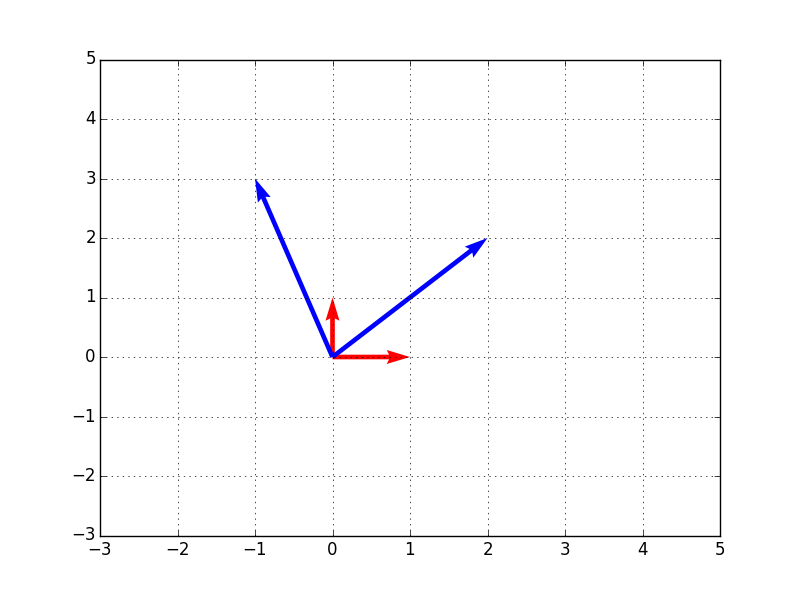
\includegraphics[width=0.75\textwidth]{6.png}
\item[(7)]
Suppose we have a matrix $A$ in row reduced echelon form:
$$A = \begin{bmatrix}
\begin{array}{c|c|c}
& 1 & B \\
\hline
& & D
\end{array}
\end{bmatrix}$$
Suppose we can inductively reduce the submatrix $D$ with column operations such that all pivots are denoted with a 1, and all other values are 0. Then we use column operations to negate out all values in $B$. Thus, $A$ can be reduced to a matrix which only has 1's in the locations of the pivots, and all other values are 0.
\item[(8)]
\begin{itemize}
\item[(a)]
Let $A = e_{ij}$, $B = e_{k\ell}$, $E = AB$. Then
$$E_{xy} = \sum_{z = 1}^n A_{xz}B_{zy}$$
Note that if $j=k$, then
$$E_{i\ell} = \sum_{z=1}^n A_{iz}B_{z\ell} = A_{ij}B_{k\ell} = 1$$
If $j \neq k$, then $E_{i\ell} = 0$. For all other $x, y$, then $E_{xy} = 0$. 
\item[(b)]
$$I = e_{11} + e_{22} + ... + e_{nn} = \sum_{i=1}^n e_{ii}$$
\item[(c)]
Denote $A^{(k)}$ the $n \times n$ matrix where for each $i$, $A^{(k)}_{ik} = A_{ik}$, and $A^{(k)}_{ij} = A_{ij}$ for $j \neq k$. Then
$$e_{ii}Ae_{jj} = e_{ii}A^{(j)} = A_{ij}e_{ii}$$
\item[(d)]
Denote $B = e_{ij}A$. If $a = i$, then for all $b$, $B_{ab} = A_{jb}$. Otherwise, $B_{ab} = 0$.

Denote $C = Ae_{ij}$. If $b = j$, then for all $a$, $C_{ab} = A_{ai}$. Otherwise, $C_{ab} = 0$.
\end{itemize}
\item[(9)]
Let $X$ be an arbitrary matrix. Let $E_1 = I + ae_{ij}$ be a type (i) matrix. Then
$$E_1X = (I + ae_{ij}X) = X + ae_{ij}X$$
Then, if $x = i$, then for all $y$, $(E_1X)_{xy} = X_{iy} + aX_{jy}$, ie. scaling row $j$ by a and adding it to row $i$. If $x \neq i$, then for all $y$, $(E_1X)_{xy} = X_{xy}$.

Let $E_2 = I + e_{ij} + e_{ji} - e_{ii} - e_{jj}$ be a type (ii) matrix. Then
$$E_2X = (I + e_{ij} + e_{ji} - e_{ii} - e_{jj})X = X + e_{ij}X + e_{ji}X - e_{ii}X - e_{jj}X$$
Then, if $x = i$, then for all $y$, $(E_2X)_{xy} = X_{iy} + X_{jy} - X_{iy} = X_{jy}$. If $x = j$, then for all $y$, $(E_2X)_{xy} = X_{jy} + X_{iy} - X_{jy} = X_{iy}$. Otherwise, $(E_2X)_{xy} = X_{xy}$. Ie. rows $i$ and $j$ are interchanged.

Let $E_3 = I + (c - 1)e_{ii}$ be a type (iii) matrix. Then
$$E_3X = (I + (c - 1)e_{ii})X = X + (c-1)e_{ii}X$$
Then, if $x = i$, then for all $y$, $(E_3X)_{xy} = X_{iy} + (c-1)X_{iy} = cX_{iy}$. Otherwise, $(E_3X)_{xy} = X_{xy}$. Ie. row $i$ is multiplied by $c$.
\item[(10)]
Let $A'$ be the row reduced echelon form of $A$. Then there exists a set of elementary matrices $E_1, ..., E_K$ such that $E_k...E_1A = A'$. If every row of $A'$ contains a pivot, then each $A'_{ii} = 1$, and  for $ i \neq j$, $A'_{ij} = 0$, ie. $A'$ is the identity. Suppose some row $i$ of $A'$ does not contain a pivot. Then every row $\geq i$ also does not contain a pivot, and in particular each such row is a row of zeros. Therefore, $A'$ has its bottom row zero.
\item[(11)]
Consider the $2 \times 2$ matrix $A$, where
$$A = \begin{bmatrix}
a & b \\
c & d
\end{bmatrix}$$
Note that if $a = c = 0$, then $A$ is not invertible. If $c = 0$, note that $d \neq 0$ (otherwise $A$ is not invertible). Then
$$\begin{bmatrix}
a & b \\
& d
\end{bmatrix} \rightarrow \begin{bmatrix}
1 & b/a \\
& d
\end{bmatrix} \rightarrow \begin{bmatrix}
1 & b/a \\
& 1
\end{bmatrix} \rightarrow \begin{bmatrix}
1 & \\
& 1
\end{bmatrix}$$
If $a = 0$, then $b \neq 0$. Then we can swap rows 1 and 2, and proceed as above (so that 4 operations total are used). If $a \neq 0$ and $c \neq 0$, then
$$\begin{bmatrix}
a & b \\
c & d
\end{bmatrix} \rightarrow \begin{bmatrix}
1 & b/a \\
c & d
\end{bmatrix} \rightarrow \begin{bmatrix}
1 & b/a \\
& d - bc/a
\end{bmatrix} \rightarrow \begin{bmatrix}
1 & b/a \\
& 1
\end{bmatrix} \rightarrow \begin{bmatrix}
1 & \\
& 1
\end{bmatrix}$$
Note with respect to the above operations that if $ad - bc = 0$, then $A$ is not invertible. So, $A$ can be reduced to the identity in 4 operations $E_1, E_2, E_3, E_4$, where some $E_i$ may be the identity operation. Then $A^{-1} = E_4E_3E_2E_1$, so $A^{-1}$ is a product of at most 4 elementary matrices.
\item[(12)]
Suppose $A$ is not invertible. Then for some elementary row operations $E_p, E_{p-1}, ..., E_1$, $A$ has reduced echelon form $A'$ such that $E_p...E_1A = A'$, and $A'$ has a bottom row of 0s. Then $AB = (E_p...E_1)^{-1}A'B$, and furthermore $A'B$ also has a bottom row of zeros. Therefore, $AB$ is cannot row reduce to the identity matrix, and therefore $AB$ is not invertible.

Thus, if $AB$ is invertible, then $A$ is invertible. Therefore, for some set of elementary matrices, $A = E_1...E_p$. Thus, $AB = E_1...E_pB \rightarrow (AB)E_p^{-1}...E_1^{-1} = B$. Since 
$$BE_1...E_p(AB)^{-1} =(AB)E_p^{-1}...E_1^{-1}E_1...E_p(AB)^{-1} = I$$
Then $B^{-1} = E_1...E_p(AB)^{-1}$, so $B$ is invertible.
\item[(13)]
Let $A$ be a $n \times m$ matrix. Then $A^\top$ is a $m \times n$ matrix, $AA^\top$ is a $n \times n$ matrix, and
$$(AA^\top)_{ij} = \sum_{k=1}^n A_{ki}A^\top_{jk} = \sum_{k=1}^n A_{ki}A_{kj}$$
Since $(AA^\top)_{ij} = (AA^\top)_{ji}$, then $AA^\top$ is symmetric.

$$(A + A^\top)_{ij} = A_{ij} + A^\top_{ii} = A_{ij} + A_{ji}$$
Since $(A + A^\top)_{ij} = (A + A^\top)_{ji}$, then $A + A^\top$ is symmetric.
\item[(14)]
\begin{itemize}
\item[(a)] 
Let $A$ be a $n \times m$ matrix and $B$ be a $m \times n$ matrix. Then
$$(B^\top A^\top)_{ij} = \sum_{k=1}^n B^\top_{ik}A^\top_{kj} = \sum_{k=1}^n B_{ki}A_{jk} = (AB)_{ji} = ((AB)^\top)_{ij}$$

And, $((A^\top)^\top)_{ij} = (A^\top)_{ji} = A_{ij}$.
\item[(b)]
$$A^\top(A^{-1})^\top = (A^{-1}A)^\top = I^\top = I$$
Thus, $(A^{-1})^\top = (A^\top)^{-1}$.
\end{itemize}
\item[(15)]
If $A$ is symmetric and invertible, then
$$(A^{-1})^\top = (A^\top)^{-1} = A^{-1}$$
Thus $A^{-1}$ is symmetric.
\item[(16)]
Suppose $AB$ is symmetric. Then
$$AB = (AB)^\top = B^\top A^\top = BA$$
Suppose $AB = BA$. Then
$$(AB)^\top = (BA)^\top = A^\top B^\top = AB$$
Thus $AB$ is symmetric.
\item[(17)]
Suppose $AX = BX$ for arbitrary $X$. Then $(A - B)X = 0$. Consider the standard column vectors $e_1, ..., e_n$, where $e_i$ has a 1 in the $i$th position as its only nonzero entry. For $e_i$, then for all $j$, $0 = ((A - B)e_i)_j = (A - B)_{ji} = A_{ji} - B_{ji} \rightarrow A_{ji} = B_{ji}$. Thus, $A = B$.
\item[(18)]
\begin{itemize}
\item[(a)] Suppose $AX = B$ has two distinct solutions $X_1, X_2$. Then $A(X_1 - X_2) = AX_1 - AX_2 = 0$, and for all $c \in \mathbb{R}$, $A(cX_1 - cX_2) = 0$. Thus, $A(X_1 + cX_1 - cX_2) = B \rightarrow X_1 + cX_1 - cX_2$ is also a solution. Therefore, $AX = B$ has infinitely many solutions.
\item[(b)]
Suppose $A = m \times n$ matrix, and let
$$X = \begin{bmatrix}
x_1 + y_1i \\
\vdots \\
x_n + y_ni
\end{bmatrix}$$
where at least one $y_i \neq 0$. Then
$$B_j = \sum_{k=1}^n A_{jk}X_k = \sum_{k=1}^n A_{jk}(x_k + y_ki)$$
Since $B_j$ is real, then
$$\sum_{k=1}^n A_{jk}y_{k} = 0$$
The above equation is satisfied when each $y_{k} = 0$. Therefore,
$$X = \begin{bmatrix}
x_1 \\
\vdots \\
x_n
\end{bmatrix}$$
is also a solution for $AX = B$.
\end{itemize}
\item[(19)]
Suppose $A$ is a $m \times 1$ matrix. Then trivially the row reduced echelon form $A'$ of $A$ solely of zeros (if $A = 0$), otherwise $A'$ has a pivot in the first row. Suppose for all $m \times n - 1$ matrices that its corresponding row reduced echelon form is uniquely determined. Suppose now that $A$ is a $m \times n$ matrix, with distinct row reduced echelon forms $B$ and $C$. Note that $A = [A' | A"], B = [B' | B"]$ and $C = [C' | C"]$, where $A', B', C'$ are $m \times n - 1$ matrices, and $A", B", C"$ are $m \times 1$ matrices. Thus, $B', C'$ are row reduced echelon forms of $A'$, and in particular $B' = C'$. So, $B" \neq C"$: in particular for some $i$, $B"_i \neq C"_i$. Consider $AX = 0$. Then $BX = CX = 0$. So, we have
$$0 = \sum_{k=1}^n B_{ik}X_k = \sum_{k=1}^n C_{ik}X_k$$
Since for $1 \leq k \leq n-1$, $B_{ik} = C_{ik}$, then
$$0 = B_{in}X_n = C_{in}X_n \rightarrow (B_{in} - C_{in})X_n = 0$$
Since $B_{in} \neq C_{in}$, then $X_n = 0$. Therefore, $B"$ and $C"$ must contain a pivot, and since $B' = C'$ the pivot must be in the same location. But then all other entries of $B"$ and $C"$ must be 0. Thus, $B" = C"$, and by contradiction $B = C$.
\end{itemize}
\section{The Matrix Transpose}
\section{Determinants}
\section{Permutation Matrices}
\section{Other Formulas for the Determinant}
\section*{Miscellaneous Problems}
\begin{description}
\item[(M.5/1)]
$$A = \begin{bmatrix}
1 & 2 \\
3 & 4
\end{bmatrix} \rightarrow \begin{bmatrix}
1 & 2 \\
0 & -2
\end{bmatrix} \rightarrow \begin{bmatrix}
1 & 2 \\
0 & 1
\end{bmatrix} \rightarrow \begin{bmatrix}
1 & 0 \\
0 & 1
\end{bmatrix}$$
$$\rightarrow A = \begin{bmatrix}
1 & 0 \\
3 & 1
\end{bmatrix}\begin{bmatrix}
1 & 0 \\
0 & -2
\end{bmatrix}\begin{bmatrix}
1 & 2 \\
0 & 1
\end{bmatrix}$$
We must now show that there does not exist a pair of elementary matrices $E_1, E_2$ such that $A = E_1E_2$, or equivalently $E_1^{-1}A = E_2$. Let $E$ be the set of all elementary matrices. We will proceed by brute force: suppose 
$$E_1 = \begin{bmatrix}
1 & c \\
0 & 1
\end{bmatrix} \rightarrow E_1^{-1} = \begin{bmatrix}
1 & -c \\
0 & 1
\end{bmatrix}$$
where $c \neq 0$. Then
$$E_1^{-1}A = \begin{bmatrix}
1 & -c \\
0 & 1
\end{bmatrix}\begin{bmatrix}
1 & 2 \\
3 & 4
\end{bmatrix} = \begin{bmatrix}
1 - 3c & 2 - 4c \\
3 & 4
\end{bmatrix} \not \in E$$
Suppose
$$E_1 = \begin{bmatrix}
1 & 0 \\
c & 1
\end{bmatrix} \rightarrow E_1^{-1} = \begin{bmatrix}
1 & 0 \\
-c & 1
\end{bmatrix}$$
where $c \neq 0$. Then
$$E_1^{-1}A = \begin{bmatrix}
1 & 0 \\
-c & 1
\end{bmatrix}\begin{bmatrix}
1 & 2 \\
3 & 4
\end{bmatrix} = \begin{bmatrix}
1 & 2 \\
3 - c & 4 - 2c
\end{bmatrix} \not \in E$$
Suppose
$$E_1 = \begin{bmatrix}
0 & 1 \\
1 & 0
\end{bmatrix} \rightarrow E_1^{-1} = \begin{bmatrix}
0 & 1 \\
1 & 0
\end{bmatrix}$$
Then
$$E_1^{-1}A = \begin{bmatrix}
0 & 1 \\
1 & 0
\end{bmatrix}\begin{bmatrix}
1 & 2 \\
3 & 4
\end{bmatrix} = \begin{bmatrix}
3 & 4 \\
1 & 2
\end{bmatrix} \not \in E$$
Suppose
$$E_1 = \begin{bmatrix}
c & 0 \\
0 & 1
\end{bmatrix} \rightarrow E_1^{-1} = \begin{bmatrix}
1/c & 0 \\
0 & 1
\end{bmatrix}$$
where $c \neq 0, 1$. Then
$$E_1^{-1}A = \begin{bmatrix}
1/c & 0 \\
0 & 1
\end{bmatrix}\begin{bmatrix}
1 & 2 \\
3 & 4
\end{bmatrix} = \begin{bmatrix}
1/c & 2/c \\
3 & 4
\end{bmatrix} \not \in E$$
Suppose
$$E_1 = \begin{bmatrix}
1 & 0 \\
0 & c
\end{bmatrix} \rightarrow E_1^{-1} = \begin{bmatrix}
c & 0 \\
0 & 1/c
\end{bmatrix}$$
where $c \neq 0, 1$. Then
$$E_1^{-1}A = \begin{bmatrix}
1 & 0 \\
0 & 1/c
\end{bmatrix}\begin{bmatrix}
1 & 2 \\
3 & 4
\end{bmatrix} = \begin{bmatrix}
1 & 2 \\
3/c & 4/c
\end{bmatrix} \not \in E$$
\item[(2)]
Let
$$A = \begin{bmatrix}
0 & -1 \\
1 & 0
\end{bmatrix}$$
Then
$$A^2 = \begin{bmatrix}
0 & -1 \\
1 & 0
\end{bmatrix}\begin{bmatrix}
0 & -1 \\
1 & 0
\end{bmatrix} = \begin{bmatrix}
-1 & 0 \\
0 & -1
\end{bmatrix} = -I$$
So, the complex number $a + bi$ can be represented by the matrix
$$\begin{bmatrix}
a & -b \\
b & a
\end{bmatrix}$$
Then, we can add two complex numbers $(a + bi) + (c + di) = (a + c) + (b + d)i$:
$$\begin{bmatrix}
a & -b \\
b & a
\end{bmatrix} + \begin{bmatrix}
c & -d \\
d & c
\end{bmatrix} = \begin{bmatrix}
a + c & -(b + d) \\
b + d & a + c
\end{bmatrix}$$
And we can multiply two complex numbers $(a + bi)(c + di) = (ac - bd) + (ad + bc)i$:
$$\begin{bmatrix}
a & -b \\
b & a
\end{bmatrix}\begin{bmatrix}
c & -d \\
d & c
\end{bmatrix} = \begin{bmatrix}
ac - bd & -(ad + bc) \\
ad + bc & ac - bd
\end{bmatrix}$$
\item[(M.7/3)]
\begin{itemize}
\item[(a)]
$$\det\begin{bmatrix}
1 & 1 & 1 \\
a & b & c \\
a^2 & b^2 & c^2
\end{bmatrix} = \det\begin{bmatrix}
b & c \\
b^2 & c^2
\end{bmatrix} - \det\begin{bmatrix}
a & c \\
a^2 & c^2
\end{bmatrix} + \det\begin{bmatrix}
a & b \\
a^2 & b^2
\end{bmatrix}$$
$$= (bc^2 - b^2c) - (ac^2 - a^2c) + (ab^2 - a^2b) = c(bc  - b^2 + a^2 - ac) + ab(b - a)$$
$$= c((a - b)(a + b) + c(b - a)) + ab(b - a) = -c(b - a)(a + b - c) + ab(b - a)$$
$$= (b - a)(ab - ac - bc + c^2) = (b - a)(a(b - c) - c(b - c)$$
$$= (b - a)(b - c)(a - c) = (b - a)(c - a)(c - b)$$
\item[(b)]
Let 
$$A = \begin{bmatrix}
1 & 1 & 1 & \cdots & 1 \\
a_1 & a_2 & a_3 & \cdots & a_k \\
a_1^2 & a_2^2 & a_3^2 & \cdots & a_k^2 \\
\vdots & \vdots & \vdots & \ddots & \vdots \\
a_1^{k-1} & a_2^{k-1} & a_3^{k-1} & \cdots & a_k^{k-1}
\end{bmatrix}$$
I claim that $\det A = \prod_{i < j}(a_j - a_i)$. Suppose $n = 2$. Then $\det A = (a_2 - a_1)$, so the statement is valid for $n = 2$. Suppose the statement is true for $n = k - 1$. Then for $n = k$,
$$\det A = \det\begin{bmatrix}
1 & 1 & 1 & \cdots & 1 \\
a_1 & a_2 & a_3 & \cdots & a_k \\
a_1^2 & a_2^2 & a_3^2 & \cdots & a_k^2 \\
\vdots & \vdots & \vdots & \ddots & \vdots \\
a_1^{k-1} & a_2^{k-1} & a_3^{k-1} & \cdots & a_k^{k-1}
\end{bmatrix}$$ 
$$= \det\begin{bmatrix}
0 & 1 - a_2/a_1 & 1 - a_3/a_1 & \cdots & 1 - a_k/a_1 \\
0 & a_2 - a_2^2/a_1 & a_3 - a_3^2/a_1 & \cdots & a_k - a_k^2/a_1 \\
0 & a_2^2 - a_2^3/a_1 & a_3^2 - a_3^3/a_1 & \cdots & a_k^2 - a_k^3/a_1 \\
\vdots & \vdots & \vdots & \ddots & \vdots \\
0 & a_2^{k-2} - a_2^{k-1}/a_1 & a_3^{k-2} - a_3^{k-1}/a_1 & \cdots & a_k^{k-2} - a_k^{k-1}/a_1 \\
a_1^{k-1} & a_2^{k-1} & a_3^{k-1} & \cdots & a_k^{k-1}
\end{bmatrix}$$
$$= \frac{1}{a_1^{k-1}}\det\begin{bmatrix}
0 & a_1 - a_2 & a_1 - a_3 & \cdots & a_1 - a_k \\
0 & a_2(a_1 - a_2) & a_3(a_1 - a_3) & \cdots & a_k(a_1 - a_k) \\
0 & a_2^2(a_1 - a_2) & a_3^2(a_1 - a_3) & \cdots & a_k^2(a_1 - a_k) \\
\vdots & \vdots & \vdots & \ddots & \vdots \\
0 & a_2^{k-2}(a_1 - a_2) & a_3^{k-2}(a_1 - a_3) & \cdots & a_k^{k-2}(a_1 - a_k) \\
a_1^{k-1} & a_2^{k-1} & a_3^{k-1} & \cdots & ^{k-1}
\end{bmatrix}$$
$$= \frac{(a_1 - a_2)(a_1 - a_3)...(a_1 - a_k)}{a_1^{k-1}}\det\begin{bmatrix}
0 & 1 & 1 & \cdots & 1 \\
0 & a_2 & a_3 & \cdots & a_k \\
0 & a_2^2 & a_3^2 & \cdots & a_k^2 \\
\vdots & \vdots & \vdots & \ddots & \vdots \\
0 & a_2^{k-2} & a_3^{k-2} & \cdots & a_k^{k-2} \\
a_1^{k-1} & a_2^{k-1} & a_3^{k-1} & \cdots & a_k^{k-1}
\end{bmatrix}$$
$$= (-1)^{k-1}(a_1 - a_2)(a_1 - a_3)...(a_1 - a_k)\det\begin{bmatrix}
1 & 1 & \cdots & 1 \\
a_2 & a_3 & \cdots & a_k \\
a_2^2 & a_3^2 & \cdots & a_k^2 \\
\vdots & \vdots & \ddots & \vdots \\
a_2^{k-2} & a_3^{k-2} & \cdots & a_k^{k-2} \\
a_2^{k-1} & a_3^{k-1} & \cdots & a_k^{k-1}
\end{bmatrix}$$
$$= \prod_{i < j}(a_j - a_i)$$
\end{itemize}
\item[(4)]
$X$ need not exist if $m > n$. For instance, let
$$A = \begin{bmatrix}
3 \\
0
\end{bmatrix}, B = \begin{bmatrix}
3 \\
1
\end{bmatrix}$$
Then $A$ has a left inverse
$$A' = \begin{bmatrix}
\frac{1}{3} & 0
\end{bmatrix}$$
Then
$$X = \begin{bmatrix}
\frac{1}{3} & 0
\end{bmatrix}\begin{bmatrix}
3 \\
1
\end{bmatrix} = [1]$$
But clearly
$$AX = \begin{bmatrix}
3 \\
0
\end{bmatrix}[1] = \begin{bmatrix}
3 \\
0
\end{bmatrix} \neq B$$
Note that if $m = n$ and $A$ has a left inverse, then $A$ also has a right inverse, and so the procedure is valid.
\item[(5)]
\begin{itemize}
\item[(a)]
Consider $A_1 = (1, 0)$ and $A_2 = (0, 1)$. Then
$$A = \begin{bmatrix}
1 & 0 \\
0 & 1
\end{bmatrix}$$
Clearly, $\det A = \text{area } P = 1$. Now consider arbitrary $A_1, A_2$. 

Suppose without loss of generality that $A_1 \mapsto A_1 + cA_2$ for some $c \neq 0$. Since $A_1$ is translated parallel to $\overline{A_2}$, then the area of the parallelogram remains constant. Accordingly, the operation corresponds to an elementary operation of the first kind, so the determinant remains unchanged.

Suppose $A_1 \mapsto A_2$ and $A_2 \mapsto A_1$. Clearly, the area remains unchanged. Accordingly, the operation corresponds to an elementary operation of the second kind, so the determinant changes by a factor of $-1$.

Suppose without loss of generality that $A_1 \mapsto cA_1$ for some $c \neq 0$. Let $\theta$ be the angle between $\overline{A_1}$ and $\overline{A_2}$. Since $|\sin\theta|$ remains constant, then the area changes by a factor of $|c|$. Accordingly, the operation corresponds to an elementary operation of the third kind, so the determinant changes by a factor of $c$.

Since we can arrive at any $A_1, A_2$ by applying a series of these operations to $(1, 0)$ and $(0, 1)$, then $|\det A| = \text{area }P$.
\item[(b)]
Consider $A_1 = (1, 0, ..., 0)$, $A_2 = (0, 1, 0, ..., 0)$, ..., $A_n = (0, ..., 0, 1)$. Then $A = I_n$. Clearly, $\det A = \text{vol } P = 1$. Now consider arbitrary $A_1, A_2, ..., A_n$. 

Suppose without loss of generality that $A_1 \mapsto A_1 + cA_2$ for some $c \neq 0$. Since $A_1$ is translated parallel to $\overline{A_2}$, then the volume of the parallelepiped remains constant. Accordingly, the operation corresponds to an elementary operation of the first kind, so the determinant remains unchanged.

Suppose withou loss of generality that $A_1 \mapsto A_2$ and $A_2 \mapsto A_1$. Clearly, the area remains unchanged. Accordingly, the operation corresponds to an elementary operation of the second kind, so the determinant changes by a factor of $-1$.

Suppose without loss of generality that $A_1 \mapsto cA_1$ for some $c \neq 0$. Let $\theta_i$ be the angle between $\overline{A_1}$ and $\overline{A_i}$, for $i \neq 1$. Since $|\sin\theta_i|$ remains constant, then the volume changes by a factor of $|c|$. Accordingly, the operation corresponds to an elementary operation of the third kind, so the determinant changes by a factor of $c$.

Since we can arrive at any $A_1, A_2, ..., A_n$ by applying a series of these operations to $(1, 0, ..., 0)$, ..., $(0, ..., 0, 1)$, then $|\det A| = \text{vol }P$.
\end{itemize}
\item[(6)]
\begin{itemize}
\item[(a)]
We will proceed by means of induction: suppose $A$ is a $1 \times 1$ matrix. Then clearly $A = LU$, where $L = A$ and $U = I_1$, and also $L$ and $U$ are unique. Suppose for all $k - 1 \times k - 1$ matrices $A'$, there exists unique $L'$ and $U'$ such that $A' = L'U'$. Now consider the $k \times k$ matrix $A$. We can express $A$ as
$$A = \begin{bmatrix}
\begin{array}{c|c}
A' & a \\
\hline
b & c
\end{array}
\end{bmatrix}$$
where $A'$ has dimensions $k - 1 \times k - 1$, $a$ has dimensions $k - 1 \times 1$, $b$ has dimensions $1 \times k - 1$, and $c$ has dimensions $1 \times 1$. I claim that if $A = LU$, then $L$ and $U$ are unique. Decomposing $L$ and $U$ into submatrices with the same dimensions as the submatrices of $A$, we can write
$$A = LU = \begin{bmatrix}
\begin{array}{c|c}
L' & d \\
\hline
e & f
\end{array}
\end{bmatrix}\begin{bmatrix}
\begin{array}{c|c}
U' & g \\ 
\hline
h & i
\end{array}
\end{bmatrix} = \begin{bmatrix}
\begin{array}{c|c}
L'U' + dh & L'g + di \\
\hline
eU' + fh & eg + fi
\end{array}
\end{bmatrix}$$
$$\begin{bmatrix}
\begin{array}{c|c}
L'U' & L'g \\
\hline
eU' & eg + fi
\end{array}
\end{bmatrix} = \begin{bmatrix}
\begin{array}{c|c}
A' & a \\
\hline
b & c
\end{array}
\end{bmatrix}$$
Note that $L'$ is lower triangular and $U'$ is upper triangular only 1s on its diagonal. Thus by the inductive hypothesis, $L'$ and $U'$ are unique. It now suffices to show that $g, e, f, i$ are unique.

Consider $L'g = a$. Consider the 1st row of $a$: $a_1 = L'_1g = L'_{11}g_1 \rightarrow g_1 = \frac{a_1}{L'_{11}}$. Suppose we can uniquely determine $g_i$ for $i < k$. For $i = k$, then $a_k = L'_kg = \sum_{j=1}^k L'_{kj}g_j \rightarrow g_k = \frac{1}{L'_{kk}}(a_k - \sum_{j=1}^{k-1}L'_{kj}g_j)$

Consider $eU' = b$. Consider the 1st column of $b$: $b_1 = eU'_1 = e_1U'_{11} \rightarrow e_1 = b_1$. Suppose we can uniquely determine $e_i$, for $i < k$. For $i = k$, then $b_k = eU'_k = \sum_{j=1}^k e_jU'_{jk} \rightarrow e_k = b_k - \sum_{j=1}^{k-1} e_jU'_{jk}$.

Consider $eg + fi = c$. Since $U_{x} = 1$ for all $x$, then $i = 1$. So, $f = c - eg = c - \sum_{i=1}^{k-1}e_1g_1$. By the uniqueness of $e$ and $g$ above, $f$ is then unique.

Since we have found unique $g, e, f, i$, then $L$ and $U$ are unique.
\item[(b)]
From part (a), then for $i, j$ where $i > j$ we have the following recursive formulae:
$$\ell_{11} = a_{11}$$
$$u_{ii} = 1$$
$$\ell_{ji} = u_{ij} = 0$$
$$\ell_{ij} = a_{ij} - \sum_{k=1}^{j-1} \ell_{ik}u_{kj}$$
$$u_{ji} = \frac{1}{\ell_{jj}}\left( a_{ji} - \sum_{k=1}^{j-1} \ell_{jk}u_{ki}\right)$$
$$\ell_{ii} = a_{ii} - \sum_{k=1}^{i-1}\ell_{ik}u_{ki}$$
Solving these formulae allows us to compute $L$ and $U$.
\item[(c)]
Consider the $m \times n$ matrix $A$. Define $A'$ to be the row-permuted form of $A$, where there eixsts a series of permutations such that we can transform $A'$ into $A"$ holding these properties:
\begin{itemize}
\item[1.] The first nonzero entry in every row is 1. This is a pivot
\item[2.]The first nonzero entry of row $i + 1$ is to the right of the first nonzero entry of $i$.
\end{itemize} 

We can use the following procedure to row reduce $A$ into a matrix $A'$:

If $n = 1$, then normalize the matrix using a Type 3 operation.

If $m = 1$, then find the first row containing a nonzero entry, normalize the entry using a Type 3 operation, and clear out the entries below that row using Type 1 operations

Find the first column that contains a nonzero entry. Find the first row in that column that contains a nonzero entry: denote this entry $a_{ij}$. Normalize this entry using a Type 3 operation. Then clear out the entries in column $j$ below row $i$ using Type 1 operations. Now inductively row reduce $A_{ij}$ to $A'_{ij}$: ie. row reduce the matrix $A$ without all columns $\leq j$, and row $i$.

Each Type 1 operation is a lower triangular matrix, and each Type 3 operation is a diagonal matrix. Therefore, letting $L$ be the sequence of Type 1 and Type 3 operations we have performed, we have $LA = A'$. Since $U = A" = PA'$ for some permutations $P$, then we have $PLA = U \rightarrow A = L^{-1}P^{-1}U$. It is easy to see that $L^{-1}$ is also a lower triangular matrix (since the inverse of a Type 1 operation that is lower triangular is also lower triangular and the inverse of a Type 3 operation is also diagonal), and the inverse of a permutation matrix is also a permutation matrix. Furthermore, since $A$ is invertible, then every column of $A"$ has a pivot, and we can transform $A"$ into the identity using a series of upper triangular Type 3 operations. Therefore, we have $A = LPU$ for a lower triangular $L$, a permutation $P$, and an upper triangular $U$.
\end{itemize}
\item[(7)]
\begin{itemize}
\item[(a)]
If $\det A \neq 0$, then $A$ is invertible. So, we have
$$X = A^{-1}B$$
Since by Cramer's Rule $A^{-1} = \frac{1}{\det A}\text{adj }A$, and since $\text{adj }A$ has integer entries (since each $\det A_{ij}$ is an integer), then $A^{-1}$ has rational entries. Since $B$ also has integer entries, then $X$ has rational entries.
\item[(b)]
Consider
$$A = \begin{bmatrix}
2 & 2 \\
0 & 1
\end{bmatrix}, B = \begin{bmatrix}
3 \\
1
\end{bmatrix}$$
Then necessarily
$$X = \begin{bmatrix}
\frac{1}{2} \\
1
\end{bmatrix}$$
$X$ is a rational solution, but there are no additional solutions, so there is not an additional integer solution.
\end{itemize}
\item[(M.10/8)]
Suppose $C = I_m - AB$ is invertible. Let $D = I_n - BA$. Consider $E = (I_n + BC^{-1}A)$. Then
$$DE = (I_n - BA)(I_n + BC^{-1}A) = I_n - BA + BC^{-1}A - BABC^{-1}A$$
$$= I_n - BA + B(C^{-1} - ABC^{-1})A = I_n - BA + B((I_m - AB)C^{-1})A$$
$$= I_n - BA + B(CC^{-1})A = I_n - BA + BA = I_n$$
Similarly,
$$ED = (I_n + BC^{-1}A)(I_n - BA) = I_n + BC^{-1}A - BA - BC^{-1}ABA$$
$$= I_n - BA + B(C^{-1} - C^{-1}AB)A = I_n - BA + B(C^{-1}(I_m - AB))A$$
$$= I_n - BA + B(C^{-1}C)A = I_n - BA + BA = I_n$$
Therefore, $D$ is invertible. We can similarly show that if $D$ is invertible, then $C$ is also invertible.
\end{description}

\chapter{Groups}

\section{Laws of Composition}
\begin{description}
\item[(1)]
\begin{itemize}
\item[(a)]
$$1 = \begin{bmatrix}
1 & 0 & 0 \\
0 & 1 & 0 \\
0 & 0 & 1
\end{bmatrix}, x = \begin{bmatrix}
0 & 1 & 0 \\
0 & 0 & 1 \\
1 & 0 & 0
\end{bmatrix}, y = \begin{bmatrix}
0 & 1 & 0 \\
1 & 0 & 0 \\
0 & 0 & 1
\end{bmatrix}$$
$$x^2 = \begin{bmatrix}
0 & 0 & 1 \\
1 & 0 & 0 \\
0 & 1 & 0
\end{bmatrix}, xy = \begin{bmatrix}
1 & 0 & 0 \\
0 & 0 & 1 \\
0 & 1 & 0
\end{bmatrix}, x^2y = \begin{bmatrix}
0 & 0 & 1 \\
0 & 1 & 0 \\
1 & 0 & 0
\end{bmatrix}$$
$$x^3 = \begin{bmatrix}
1 & 0 & 0 \\
0 & 1 & 0 \\
0 & 0 & 1
\end{bmatrix}, y^2 = \begin{bmatrix}
1 & 0 & 0 \\
0 & 1 & 0 \\
0 & 0 & 1
\end{bmatrix}, yx = \begin{bmatrix}
0 & 0 & 1 \\
0 & 1 & 0 \\
1 & 0 & 0
\end{bmatrix} = x^2y$$
\item[(b)]
\begin{tabular}{| c || c | c | c | c | c | c |}
\hline
& 1 & $x$ & $x^2$ & $y$ & $xy$ & $x^2y$ \\
\hline \hline
1 & 1 & $x$ & $x^2$ & $y$ & $xy$ & $x^2y$ \\
\hline
$x$ & $x$ & $x^2$ & 1 & $xy$ & $x^2y$ & $y$ \\
\hline
$x^2$ & $x^2$ & 1 & $x$ & $x^2y$ & $y$ & $xy$ \\
\hline
$y$ & $y$ & $x^2y$ & $xy$ & 1 & $x^2$ & $x$ \\
\hline
$xy$ & $xy$ & $y$ & $x^2y$ & $x$ & 1 & $x^2$ \\
\hline
$x^2y$ & $x^2y$ & $xy$ & $y$ & $x^2$ & $x$ & $x^3$ \\
\hline
\end{tabular}
\end{itemize}
\item[(2)]
\begin{itemize}
\item[(a)]
Let $A, B, C \in GL(\mathbb{R})$. 

Note that $\det(AB) = \det(A)\det(B) \neq 0$, so $AB \in GL(\mathbb{R})$, so multiplication is a law of composition of $GL(\mathbb{R})$.

Further for $1 \leq i,j \leq n$,
$$((AB)C)_{ij} = \sum_{k=1}^n (AB)_{ik}c_{kj} = \sum_{k=1}^n\left(\sum_{m=1}^n a_{im}b_{mk}\right)c_{kj} $$
$$= \sum_{k=1}^n\sum_{m=1}^n a_{im}b_{mk}c_{kj} = \sum_{m=1}^na_{im}\left(\sum_{k=1}^n b_{mk}c_{kj}\right)$$
$$= \sum_{m=1}^na_{im}(BC)_{mj} = (A(BC))_{ij}$$
So multiplication is associative on $GL(\mathbb{R})$.

Note that $I \in GL(\mathbb{R})$, and $AI = IA = A$, so $GL(\mathbb{R})$ contains the identity matrix.

Since $\det A \neq 0$, then $A$ is invertible. Necessarily, $\det A^{-1} \neq 0$, and $AA^{-1} = A^{-1}A = I$, so $A$ has an inverse. 

Thus, $GL(\mathbb{R})$ is a group.
\item[(b)]
Let $X, Y, Z \in S_n$. Then for some $a, b, c \in 1...n$, $(XY)(a) = X(Y(a)) = X(b) = c$. So we have a law of composition of $S_n$.

Further,
$$((XY)Z)(a) = (XYZ)(a) = (X(YZ))(a)$$
So the law of composition is associative.

Note that $i \in S_n$, and $(Xi)(a) = X(i(a)) = X(a) = b$, and $(iX)(a) = i(X(a)) = i(b) = b$. so $S_n$ contains the identity permutation.

Suppose $X$ is a permutation such that $X(a) = b, X(b) = c$. Then there exists a permutation $Y$ such that $Y(b) = a, Y(c) = b$. So then $(XY)(b) = X(Y(b)) = X(a) = b$, and $(YX)(b) = Y(X(b)) = Y(c) = b$. Thus $X$ is invertible, and its inverse is $Y$.
\end{itemize}
\item[(3)]
Let $T = \left\lbrace s \in S | \text{\emph{s} is invertible} \right\rbrace$. Note that $I \in T$, since $II = I$. Let $t \in T$. $t$ is invertible, and has inverse $w$. Since $tw = I$, and $wt = I$, then $w$ is also invertible with inverse $t$. Thus, $w \in T$. Thus, since $T$ has an associative law of composition and the identity, then $T$ is a group.
\item[(4)]
$$xyz^{-1}w = 1 \rightarrow yz^{-1}w = x^{-1} \rightarrow yz^{-1} = x^{-1}w^{-1} \rightarrow y = x^{-1}w^{-1}z$$
\item[(5)]
$$xyz = 1 \rightarrow yz = x^{-1} \rightarrow yzx = 1$$
It does not follow that $yxz = 1$. Let $a = x, b = y, c = xy$. Then $abc = 1$. But $bac = yxxy = yx^2y = yyx = y^2x = x \neq 1$.
\item[(6)]
$$(abcd), a(bcd), (abc)d, (ab)(cd), (ab)cd, a(bc)d, ab(cd), abcd$$
\item[(7)]
Let $a, b, c \in S$. Then
$$(ab)c = ac = a = ab = a(bc)$$
Thus, the law of composition is associative.
\item[(8)]
Let $$A = \begin{bmatrix}
0 & 1 \\
1 & 0
\end{bmatrix}, B = \begin{bmatrix}
1 & 1 \\
0 & 0
\end{bmatrix}$$
Note that
$$A^{-1} = \begin{bmatrix}
0 & 1 \\
1 & 0
\end{bmatrix}$$
So
$$A^{-1}B = \begin{bmatrix}
0 & 0 \\
1 & 1
\end{bmatrix}$$
But
$$BA^{-1} = \begin{bmatrix}
1 & 1 \\
0 & 0
\end{bmatrix}$$
So $A^{-1}B \neq BA^{-1}$
\item[(9)]
$$ab = a \rightarrow a^{-1}ab = a^{-1}a \rightarrow b = 1$$
$$ab = 1 \rightarrow a^{-1}ab = a^{-1} \rightarrow b = a^{-1}$$
\item[(10)]
$$ax = b \rightarrow x = a^{-1}b$$
Since $a, b$ are distinct elements, then $x$ is unique.
\item[(11)]
Let $a, b, c \in G^\circ$. Since $a \circ b = ba \in G$, then $\circ$ is a law of composition in $G$. And,
$$(a \circ b) \circ c = (ba) \circ c = cba = (cb)a = a \circ (cb) = a \circ (b \circ c)$$
So $\circ$ is associative.

Since $I \in G$, then $a \circ I = Ia = a = aI = I \circ a$, so $I \in G^\circ$.

Let $a^{-1}$ be the inverse of $a$ in $G$. Then
$$a \circ a^{-1} = a^{-1}a = I = aa^{-1} = a^{-1} \circ a$$

So therefore $a$ has an inverse in $G^\circ$, namely $a^{-1}$. Thus $G^\circ$ is a group.
\end{description}
\end{document}